\documentclass[UTF8, xcolor=table]{beamer}
\usepackage[BoldFont,SlantFont]{xeCJK}
\setCJKmainfont[BoldFont={Adobe Heiti Std},ItalicFont={Adobe Kaiti Std}]{AdobeSongStd-Light}
 \setCJKmainfont[BoldFont={Adobe Heiti Std},ItalicFont={Adobe Kaiti Std}]{SimSum} %Windows先编译使用这个字体

\usepackage{latexsym,amssymb,amsmath,amsbsy,amsopn,amstext,xcolor,multicol}
\usepackage{graphicx,wrapfig,fancybox}
\usepackage{pgf,pgfarrows,pgfnodes,pgfautomata,pgfheaps,pgfshade}
\usepackage{thubeamer}
\usepackage[backend=bibtex,sorting=none]{biblatex} % [参考文献格式](https://www.sharelatex.com/blog/2013/07/31/getting-started-with-biblatex.html) %mac IEEE not found
\usepackage{array}
\usepackage{bm}
\usepackage{caption}
\RequirePackage[font=footnotesize]{subcaption}
\usepackage{multirow}
\usepackage{booktabs}
\usepackage{tikz}
%\usepackage{tikzscale}
\usepackage{animate}

\defbibheading{bibliography}[\bibname]{} %avoid printbibliography 自动生成目录
\addbibresource{../main.bib}
\setbeamertemplate{bibliography item}[text] 

\usepackage{boxedminipage} %for: bvh border
\def\fourgraphicswidth{0.35} %0.3\textwidth

\usepackage{algorithm} %%format of the algorithm
\usepackage{algpseudocode}
\floatname{algorithm}{算法}
\renewcommand{\algorithmicrequire}{\textbf{输入:}} % Use Input in the format of Algorithm
\renewcommand{\algorithmicensure}{\textbf{输出:}} % UseOutput in the format of Algorithm
\algrenewcommand{\algorithmiccomment}[1]{ $//$ #1}

\usepackage{listings}
\renewcommand\lstlistingname{代码}
\renewcommand\lstlistlistingname{代码}

\lstset{framexleftmargin=1.4em,
        xleftmargin=1.8em,
        basicstyle=\ttfamily\small,
        %frame=shadowbox, numberstyle=\tiny, breaklines=true,
        frame=single,
        numberstyle=\tiny, breaklines=true,
        keywordstyle=\color{blue!70}\bfseries,
        %commentstyle=\color{red!50!green!50!blue!50},
        rulesepcolor=\color{red!20!green!20!blue!20},
        numbers=none,fontadjust=true}
\lstdefinelanguage{shader}{morekeywords={uniform, layout, uniform, vec2, vec3, vec4, in, out, gl_Position, dot, flat, int ,float, gl_VertexID, xyz, w, x, y, z, location, version, sampler2DRect, bgr, gl_FragData, texture2DRect, gl_TexCoord,for,xy},morecomment=[l]{//}}

\begin{document}

\setbeamerfont{footnote}{size=\tiny}
\setbeamerfont{caption}{size=\scriptsize}
\setbeamertemplate{caption}[numbered]
\setbeamerfont{subsection in toc}{size=\footnotesize}
\renewcommand*{\bibfont}{\footnotesize}

\graphicspath{{../}}

\title[融合长短记忆神经网络与卷积特征学习的图像语义分割]{中山大学本科毕业论文演示文稿非正式模版}
\author[陈冠英]{}%{(申请中山大学工学学士学位论文答辩报告)\\ \vskip 20pt 学~~~~~~生:陈~冠~英}
\institute[中山大学~电子信息与工程学院~\&~自动化]{}%{\small \vskip 38pt 电子信息与工程学院~自动化}
\date{} %{\small \vskip -17pt二〇一六年五月}

%% make title %%
\frame{
	\titlepage
	\vspace{-23mm}
	\begin{figure}[h]
		\centering
		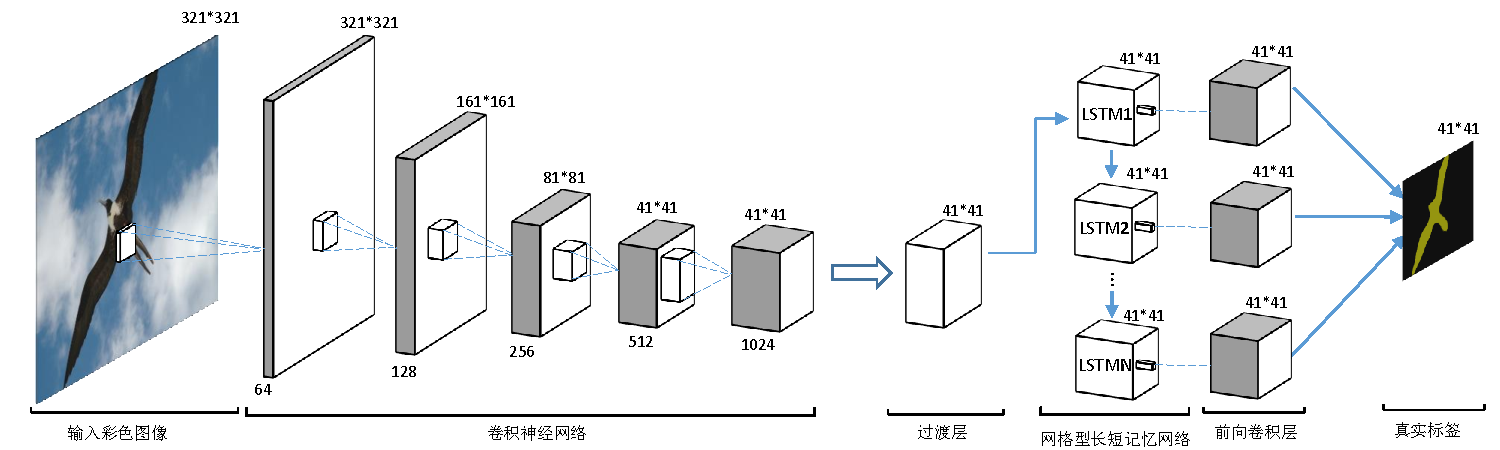
\includegraphics[width=\textwidth]{image/illustration/networkstructure.pdf}
	\end{figure}
}

\frame {
	\frametitle{目录}
	%\begin{multicols}{2}
	\tableofcontents[sections={<1-7>}]
}

%%
% 引言或背景
% 引言是论文正文的开端,应包括毕业论文选题的背景、目的和意义;对国内外研究现状和相关领域中已有的研究成果的简要评述;介绍本项研究工作研究设想、研究方法或实验设计、理论依据或实验基础;涉及范围和预期结果等。要求言简意赅,注意不要与摘要雷同或成为摘要的注解。
% modifier: 黄俊杰(huangjj27, 349373001dc@gmail.com)
% update date: 2017-04-15
%%

\chapter{绪论}
%定义,过去的研究和现在的研究,意义,与图像分割的不同,going deeper
\label{cha:introduction}
\section{选题背景与意义}
\label{sec:background}
% What is the problem
% why is it interesting and important
% Why is it hards, why do naive approaches fails
% why hasn't it been solved before
% what are the key components of my approach and results, also include any specific limitations,do not repeat the abstract
%contribution
引言是论文正文的开端,应包括毕业论文选题的背景、目的和意义;对国内外研究现状和相关领域中已有的研究成果的简要评述;介绍本项研究工作研究设想、研究方法或实验设计、理论依据或实验基础;涉及范围和预期结果等。要求言简意赅,注意不要与摘要雷同或成为摘要的注解。

\section{国内外研究现状和相关工作}
\label{sec:related_work}
对国内外研究现状和相关领域中已有的研究成果的简要评述。
\section{本文的论文结构与章节安排}

\label{sec:arrangement}

本文共分为六章,各章节内容安排如下:

第一章绪论。简单说明了本文章的选题背景与意义。

第二章为本科生毕业论文写作与印制规范。本章节就学校的规范,逐点进行描述,并给出来了相关例子说明本模板在格式上的正确性。

第三章为本模板的使用说明。

第四章为可用的\LaTeX 的代码段方便大家进行编辑。

第五、六章是本文的最后两章,作为空白章节例子。


\chapter{简单的使用例子}
\label{cha:example}

\section{深度学习方法处理图像}








\section{图像的插入}
\subsection{镶嵌在文中的图像}
\label{sec:Images}
\begin{wrapfigure}{r}{0.5\linewidth}
	\centering
	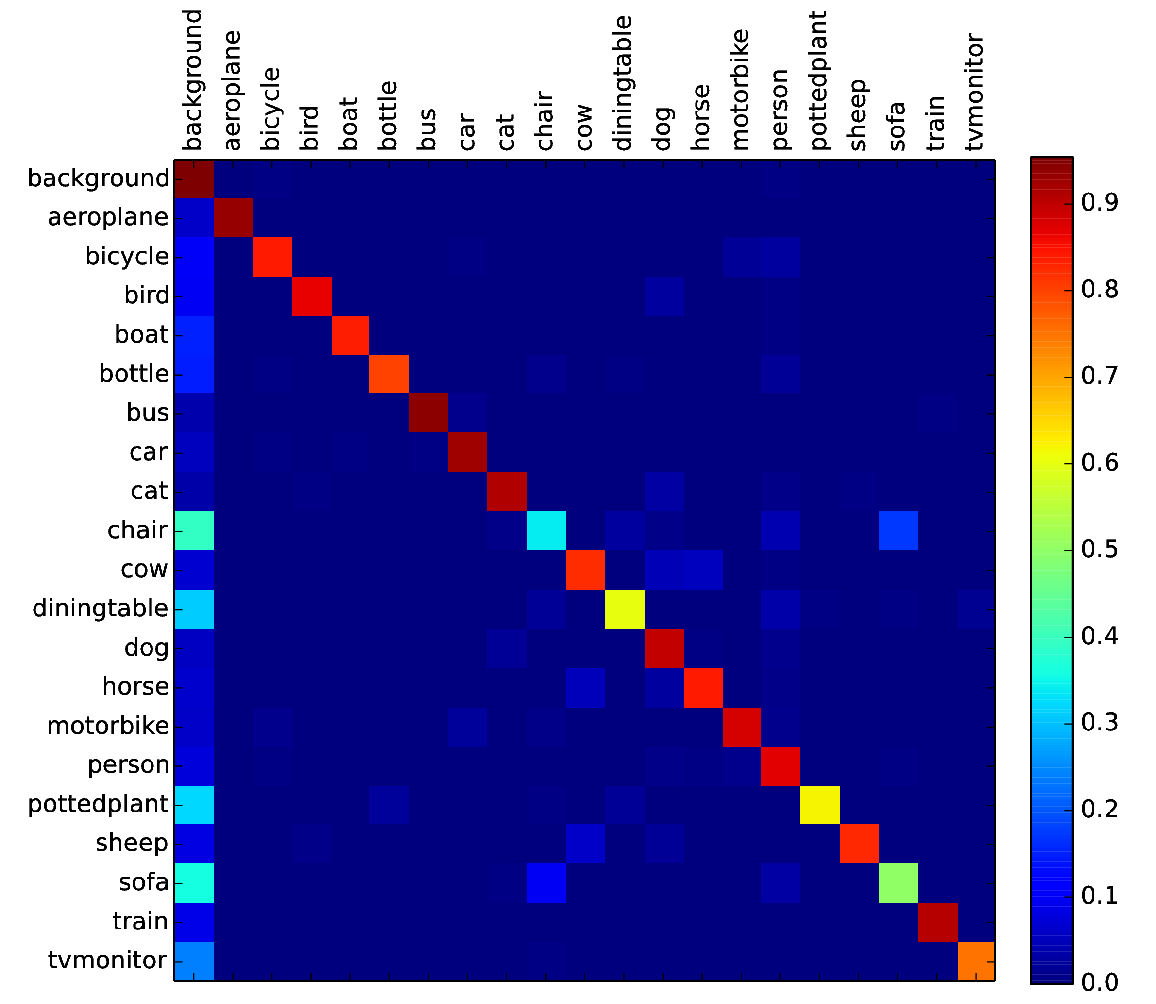
\includegraphics[width=0.5\textwidth]{image/result/confusion.pdf}
	\caption{镶嵌在文中的图像}
	\label{fig:confusion}
\end{wrapfigure}
论文主体是毕业论文的主要部分,必须言之成理,论据可靠,严格遵循本学科国际通行的学术规范。在写作上要注意结构合理、层次分明、重点突出,章节标题、公式图表符号必须规范统一。论文主体的内容根据不同学科有不同的特点,一般应包括以下几个方面: (1)毕业论文(设计)总体方案或选题的论证; (2)毕业论文(设计)各部分的设计实现,包括实验数据的获取、数据可行性及有效性的处理与分析、各部分的设计计算等; (3)对研究内容及成果的客观阐述,包括理论依据、创新见解、创造性成果及其改进与实际应用价值等; (4)论文主体的所有数据必须真实可靠,凡引用他人观点、方案、资料、数据等,无论曾否发表,无论是纸质或电子版,均应详加注释。自然科学论文应推理正确、结论清晰;人文和社会学科的论文应把握论点正确、论证充分、论据可靠,恰当运用系统分析和比较研究的方法进行模型或方案设计,注重实证研究和案例分析,根据分析结果提出建议和改进措施等。
\subsection{单张图像的插入}
\begin{figure}[h]
	\centering
	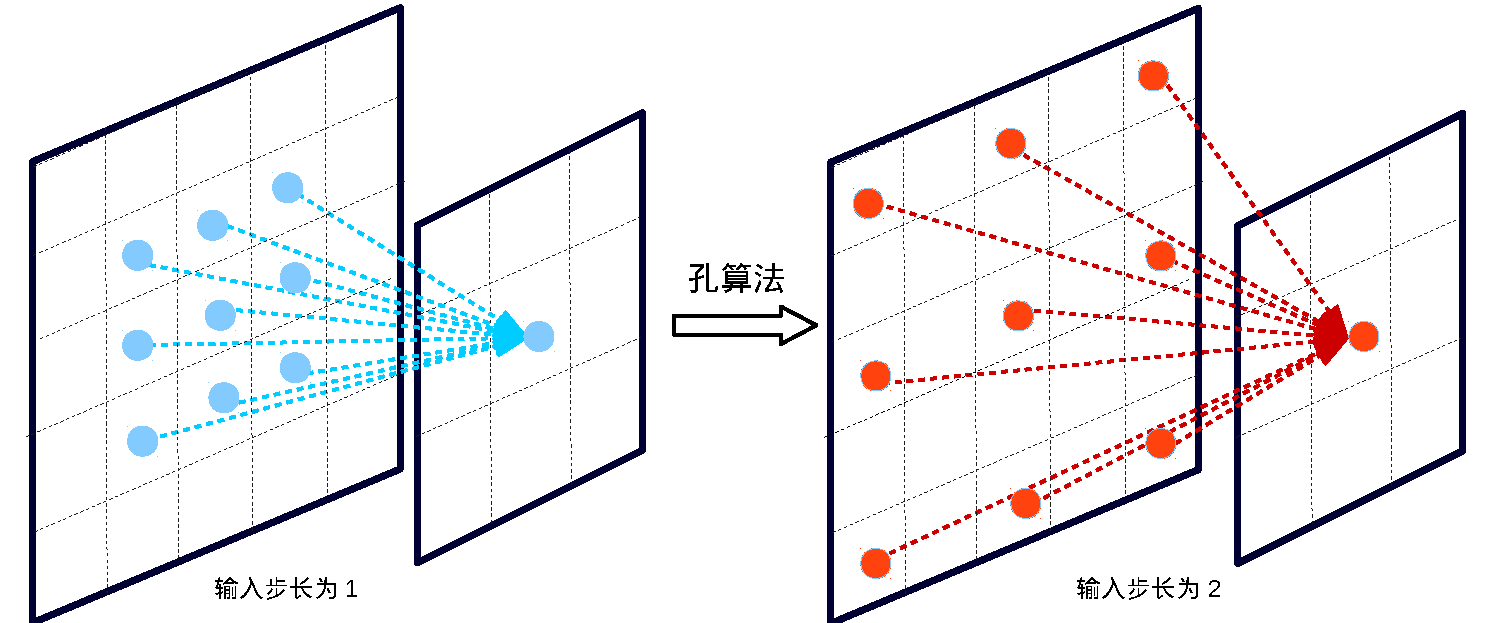
\includegraphics[width=0.5\textwidth]{image/illustration/hole.pdf}
	\caption{单张图像}
 	\label{fig:hole}
\end{figure}


\subsection{多张图像的并排插入}
\label{sub:多张图像的并排插入}
\begin{figure}[h!]%文中的Grid-LSTM模型做的语义图像分割的例子
	\centering
	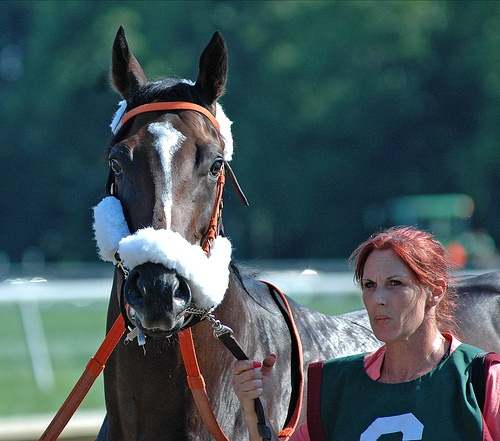
\includegraphics[width=.2\textwidth,height=.15\textwidth]{image/example/2007_000799.jpg}
	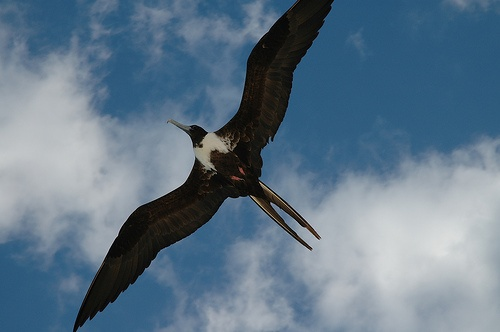
\includegraphics[width=.2\textwidth,height=.15\textwidth]{image/example/2007_002094.jpg}
	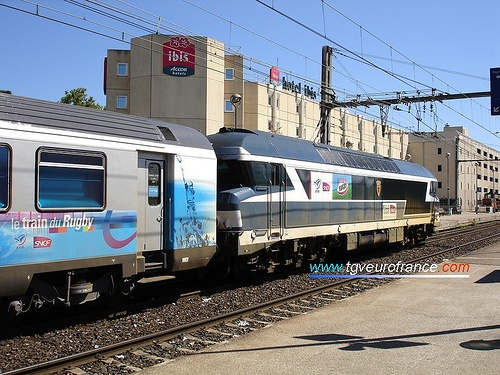
\includegraphics[width=.2\textwidth,height=.15\textwidth]{image/example/2007_004483.jpg}
	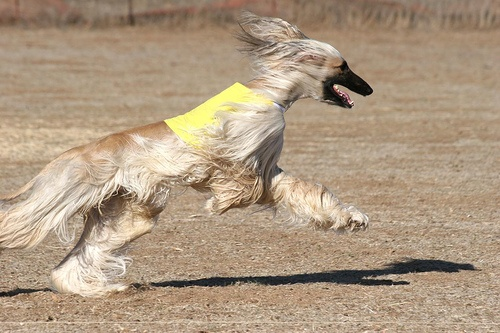
\includegraphics[width=.2\textwidth,height=.15\textwidth]{image/example/2007_003194.jpg}
	\\
	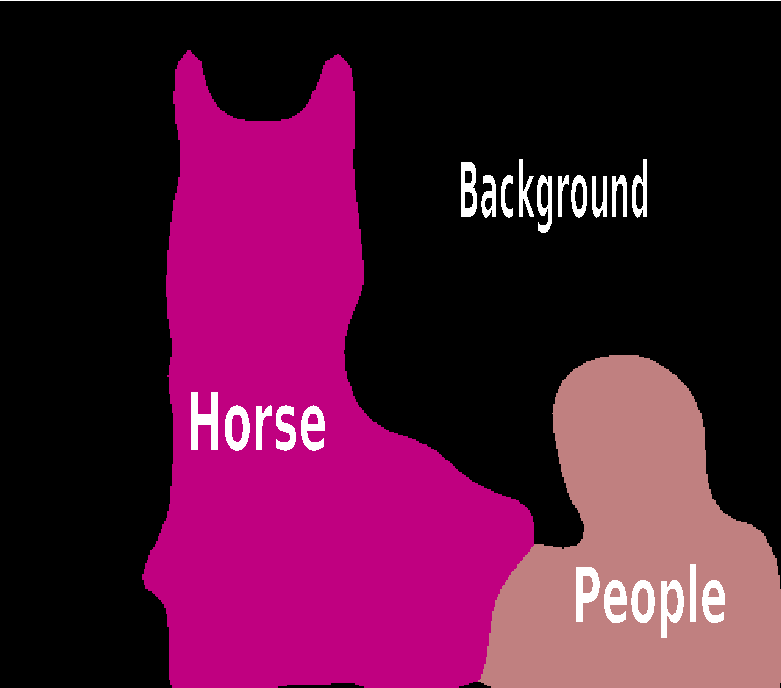
\includegraphics[width=.2\textwidth,height=.15\textwidth]{image/example/2007_000799.pdf}
	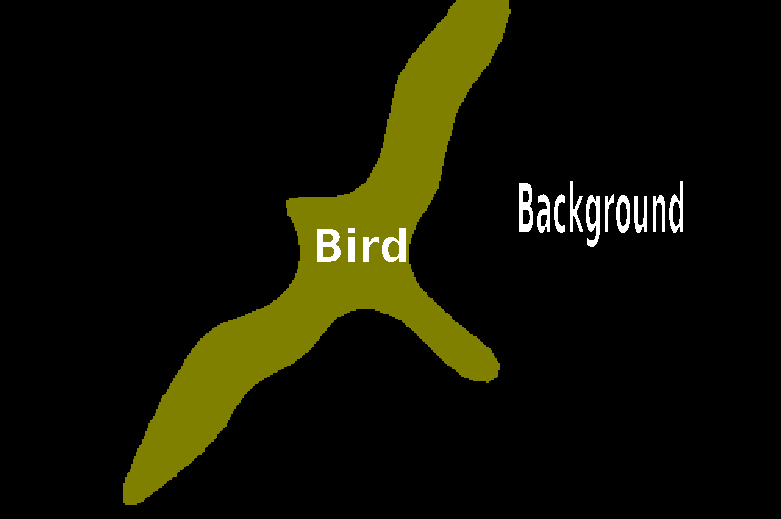
\includegraphics[width=.2\textwidth,height=.15\textwidth]{image/example/2007_002094.pdf}
	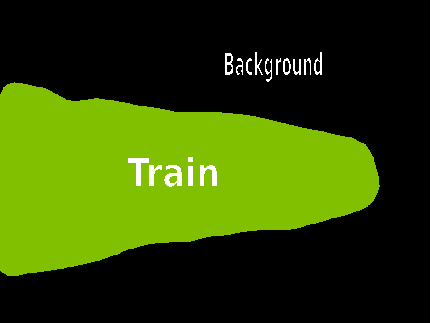
\includegraphics[width=.2\textwidth,height=.15\textwidth]{image/example/2007_004483.pdf}
	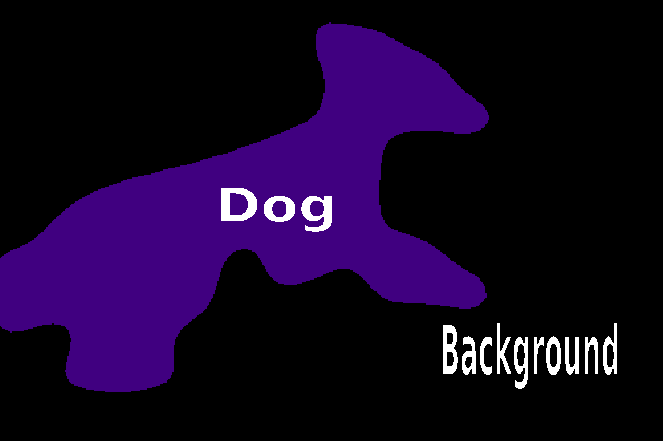
\includegraphics[width=.2\textwidth,height=.15\textwidth]{image/example/2007_003194.pdf}
	\caption{并排的多张图像}
	\label{fig:example1}
\end{figure}
\endinput

\begin{figure}[h]
\centering
	\makebox[0.11\textwidth]{\scriptsize 图像}
	\enspace
	\makebox[0.11\textwidth]{\scriptsize 真值}
	\enspace
	\makebox[0.11\textwidth]{\scriptsize CNN+5LSTM\textbf{1}}
	\enspace\thinspace
	\makebox[0.11\textwidth]{\scriptsize CNN+5LSTM\textbf{2}}
	\enspace\thinspace
	\makebox[0.11\textwidth]{\scriptsize CNN+5LSTM\textbf{3}}
	\enspace\thinspace
	\makebox[0.11\textwidth]{\scriptsize CNN+5LSTM\textbf{4}}
	\enspace\thinspace
	\makebox[0.11\textwidth]{\scriptsize CNN+5LSTM\textbf{5}}\\
	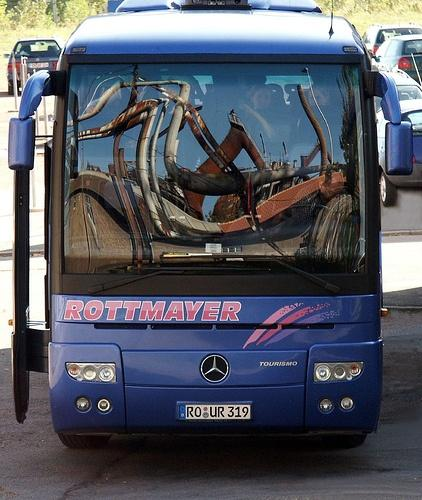
\includegraphics[width=0.11\textwidth]{image/improvement/2007_000663.jpg}
	\enspace\thinspace %\hfill
	
\includegraphics[width=0.11\textwidth]{image/improvement/2007_000663.png}
	\enspace\thinspace
	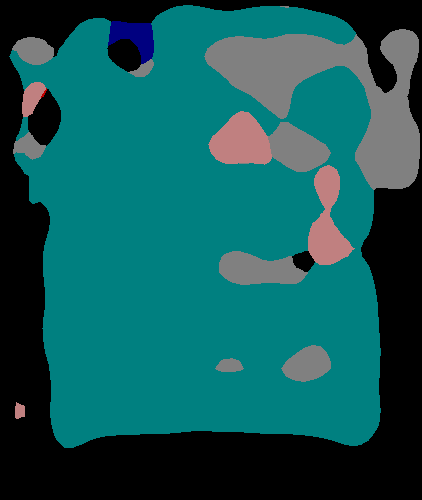
\includegraphics[width=0.11\textwidth]{image/improvement/2007_000663_1.png}
	\enspace\thinspace
	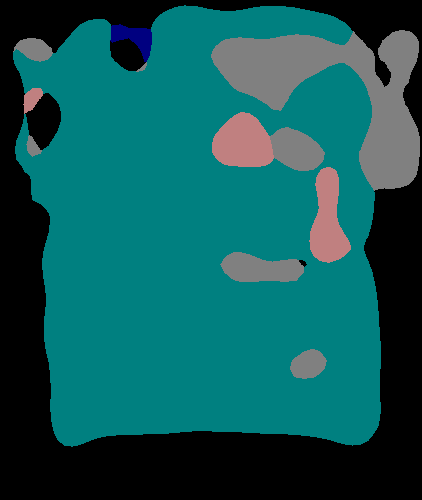
\includegraphics[width=0.11\textwidth]{image/improvement/2007_000663_2.png}
	\enspace\thinspace
	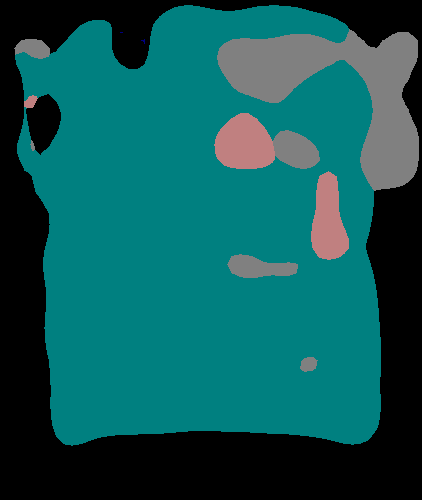
\includegraphics[width=0.11\textwidth]{image/improvement/2007_000663_3.png}
	\enspace\thinspace
	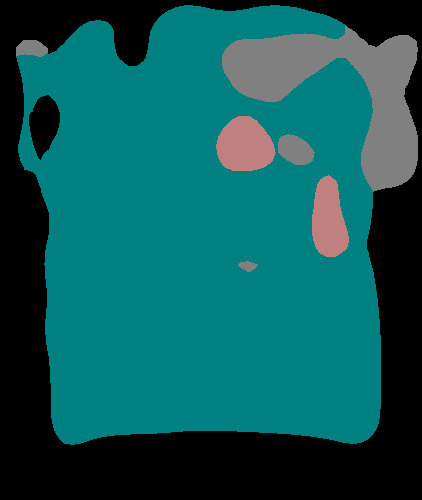
\includegraphics[width=0.11\textwidth]{image/improvement/2007_000663_4.png}
	\enspace\thinspace
	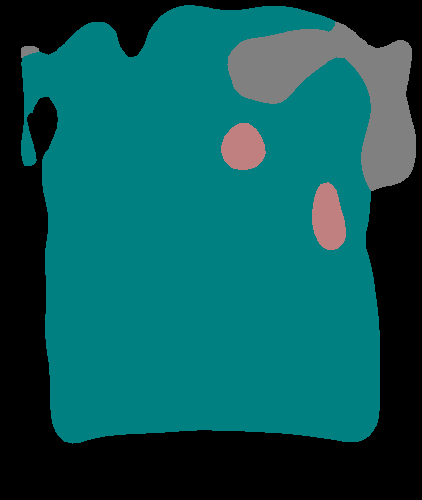
\includegraphics[width=0.11\textwidth]{image/improvement/2007_000663_5.png}
	\enspace\thinspace
	\caption{并排的多张图像加各自的注解}
	\label{fig:improvement}
\end{figure}


\subsection{两列图像的插入}
\label{sec:complex}
\begin{figure}[h!] % image examples & compare
	\begin{subfigure}{0.55\textwidth}
		\makebox[0.18\textwidth]{\scriptsize Grid-5LSTM}
		\makebox[0.18\textwidth]{\scriptsize FCN-8s\cite{long2015fully}}
		\makebox[0.18\textwidth]{\scriptsize SDS\cite{hariharan2014simultaneous}}
		\makebox[0.18\textwidth]{\scriptsize 真值}
		\makebox[0.18\textwidth]{\scriptsize 图像} \\
		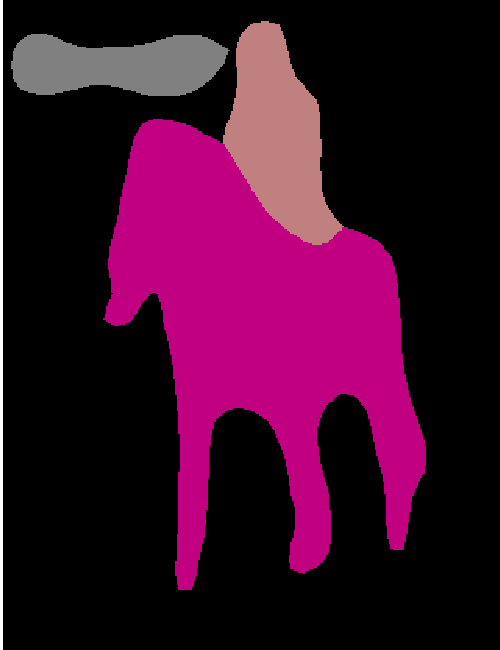
\includegraphics[width=0.18\textwidth]{image/result/compare/my_horse.pdf}
		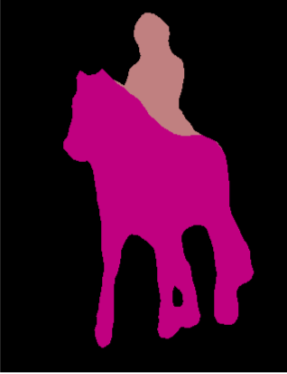
\includegraphics[width=0.18\textwidth]{image/result/compare/fcn_horse.png}
		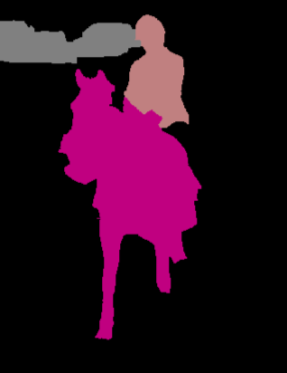
\includegraphics[width=0.18\textwidth]{image/result/compare/sds_horse.png}
		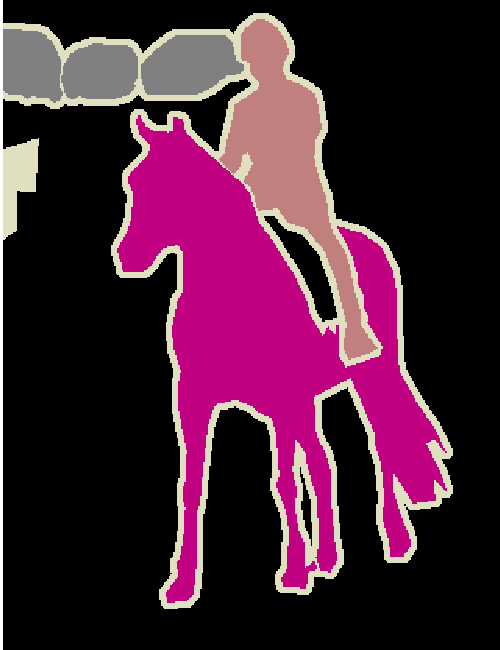
\includegraphics[width=0.18\textwidth]{image/result/compare/gt_horse.pdf}
		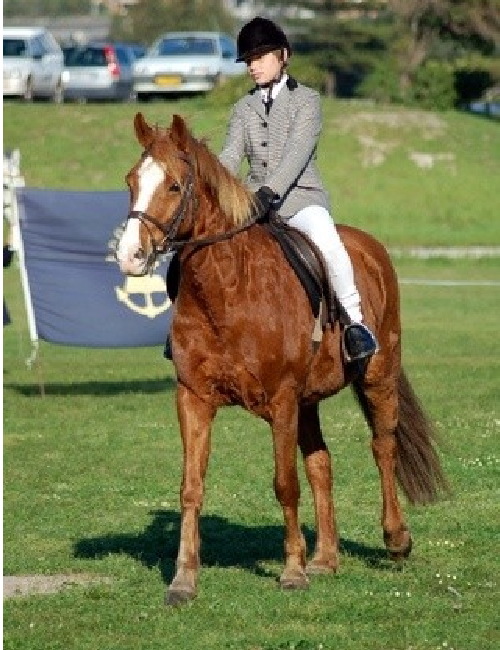
\includegraphics[width=0.18\textwidth]{image/result/compare/im_horse.pdf}
		\\
		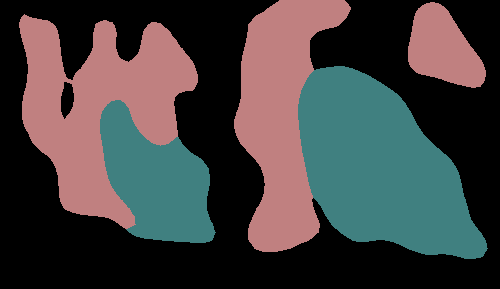
\includegraphics[width=0.18\textwidth]{image/result/compare/my_motor.png}
		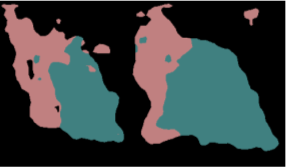
\includegraphics[width=0.18\textwidth]{image/result/compare/fcn_motor.png}
		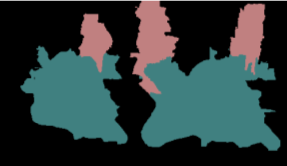
\includegraphics[width=0.18\textwidth]{image/result/compare/sds_motor.png}
		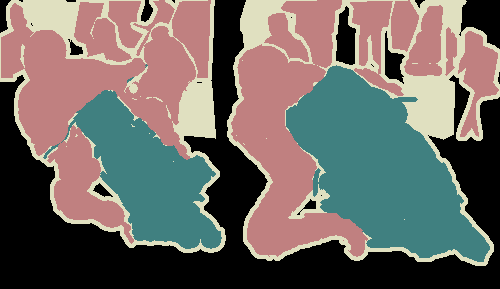
\includegraphics[width=0.18\textwidth]{image/result/compare/2007_005173.png}
		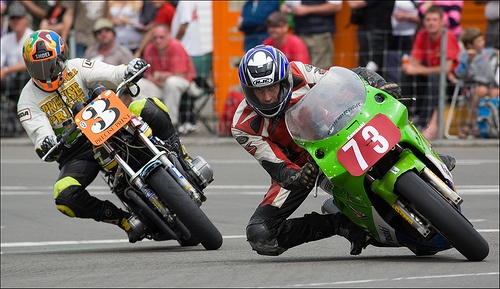
\includegraphics[width=0.18\textwidth]{image/result/compare/2007_005173.jpg}
		\\
		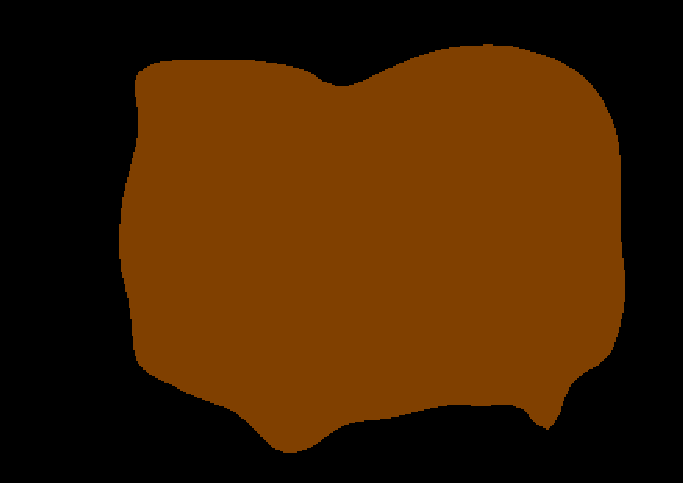
\includegraphics[width=0.18\textwidth]{image/result/compare/my_sheep.pdf}
		
\includegraphics[width=0.18\textwidth]{image/result/compare/fcn_sheep.png}
		
\includegraphics[width=0.18\textwidth]{image/result/compare/sds_sheep.png}
		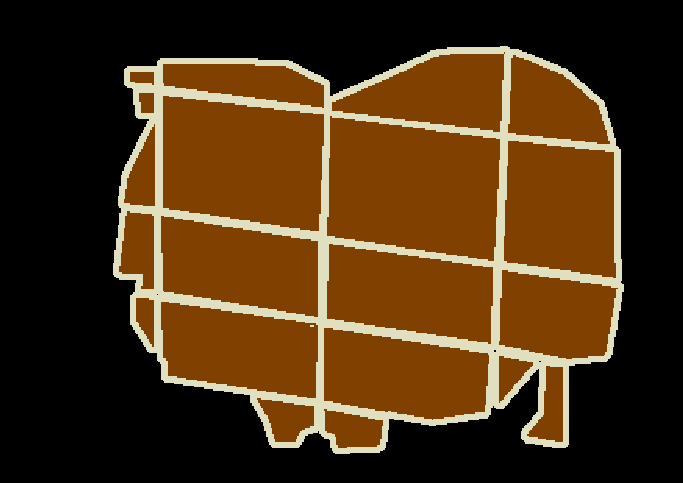
\includegraphics[width=0.18\textwidth]{image/result/compare/gt_sheep.pdf}
		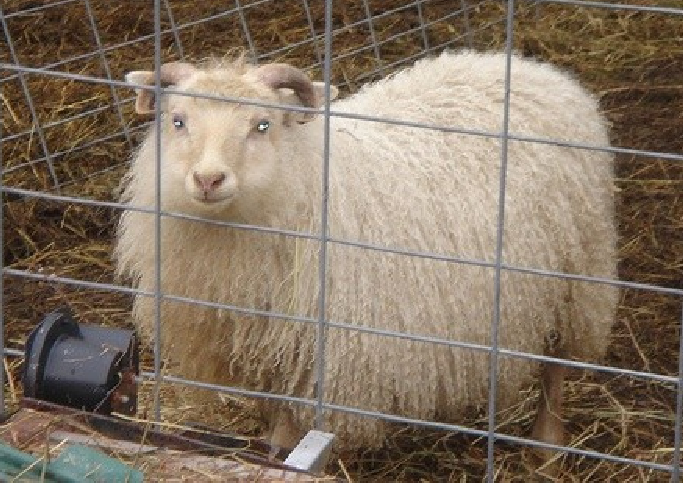
\includegraphics[width=0.18\textwidth]{image/result/compare/im_sheep.pdf}
		\\
		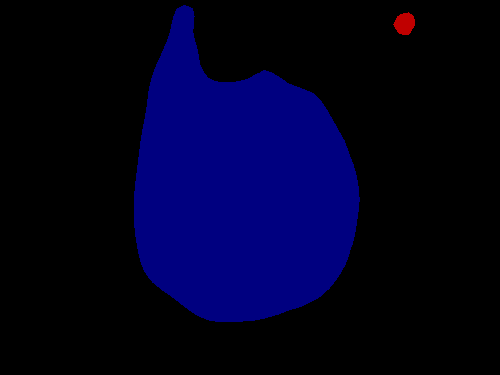
\includegraphics[width=0.18\textwidth]{image/result/compare/my_boat.png}
		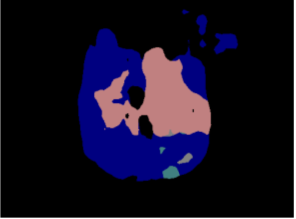
\includegraphics[width=0.18\textwidth]{image/result/compare/fcn_boat.png}
		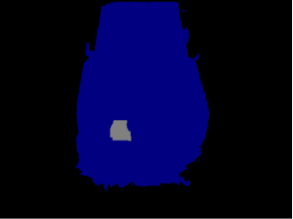
\includegraphics[width=0.18\textwidth]{image/result/compare/sds_boat.png}
		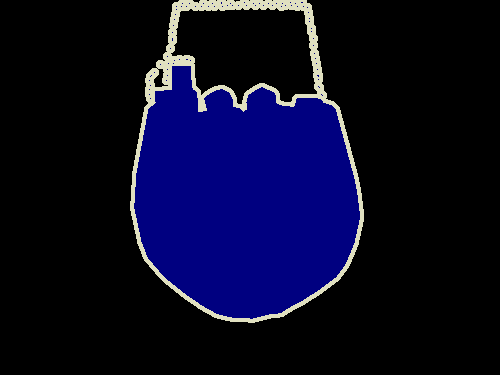
\includegraphics[width=0.18\textwidth]{image/result/compare/2007_004241.png}
		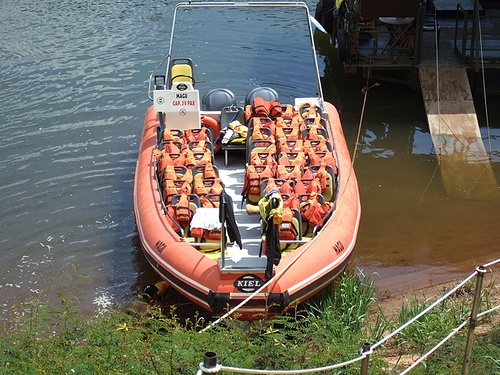
\includegraphics[width=0.18\textwidth]{image/result/compare/2007_004241.jpg}
		\caption{左边的图像}
		\label{fig:compare1}
	\end{subfigure}
	\begin{subfigure}{0.4\textwidth}
		\centering
%		\makebox[0.3\textwidth]{} \\
%		\makebox[0.3\textwidth]{} \\
		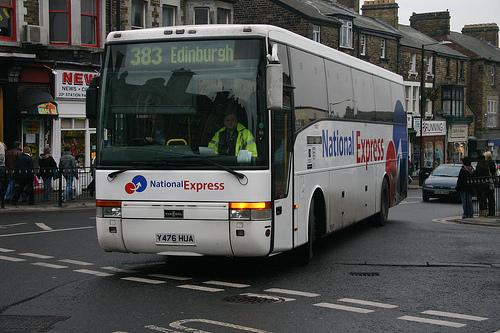
\includegraphics[width=0.25\textwidth]{image/result/compare/2010_005284.jpg}
		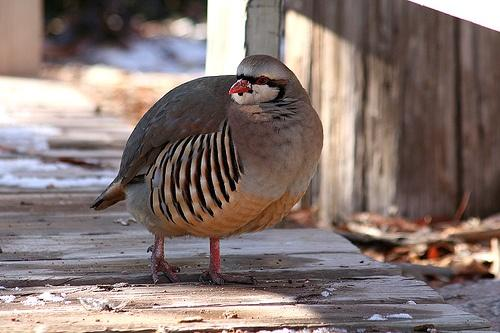
\includegraphics[width=0.25\textwidth]{image/result/compare/2007_003349.jpg}
		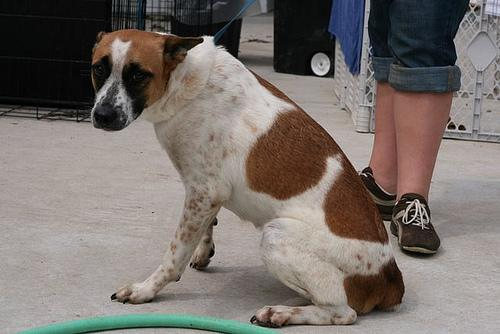
\includegraphics[width=0.25\textwidth]{image/result/compare/2009_004507.jpg} 
		\\
		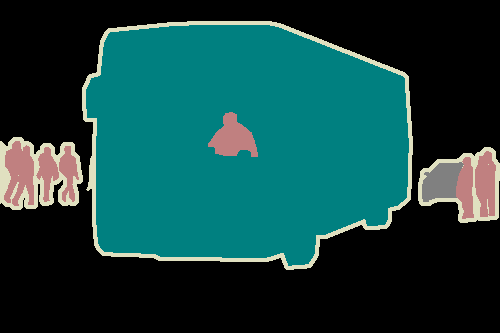
\includegraphics[width=0.25\textwidth]{image/result/compare/2010_005284.png}
		
\includegraphics[width=0.25\textwidth]{image/result/compare/2007_003349.png}
		
\includegraphics[width=0.25\textwidth]{image/result/compare/2009_004507.png} \\
		
\includegraphics[width=0.25\textwidth]{image/result/compare/zoom_bus.png}
		
\includegraphics[width=0.25\textwidth]{image/result/compare/zoom_bird.png}
		
\includegraphics[width=0.25\textwidth]{image/result/compare/zoom_dog.png} \\
		
\includegraphics[width=0.25\textwidth]{image/result/compare/deeplab_bus.png}
		
\includegraphics[width=0.25\textwidth]{image/result/compare/deeplab_bird.png}
		
\includegraphics[width=0.25\textwidth]{image/result/compare/deeplab_dog.png} \\
		\includegraphics[width=0.25\textwidth]{image/result/compare/my_bus.png}
		\includegraphics[width=0.25\textwidth]{image/result/compare/my_bird.png}
		\includegraphics[width=0.25\textwidth]{image/result/compare/my_dog.png} 
		\caption{右边的图像}
		\label{fig:compare2}
	\end{subfigure}
	\caption{复杂的两列对象的插入}
	\label{fig:complex}
\end{figure}


\clearpage

\section{表格的插入}
\label{sec:tables}
\begin{table}[h] %voc table result
	\centering
		\begin{tabular}{*{4}{c}}
			\toprule
	 		Method & Pixel Acc. & Mean Acc. & Mean Iu.\\
			\midrule
			Liu等人\cite{liu2011sift}  & 76.7 & - & -\\
		Tighe等人\cite{tighe2013finding}  & 78.6 & 39.2 & -\\
			FCN-16s\cite{long2015fully} & 85.2 & \textbf{51.7} & 39.5\\
			Deeplab-LargeFOV\cite{chen14semantic} & 85.6 & 51.2 & 39.7\\
			\midrule
			Grid-LSTM5 & \textbf{86.2} & 51.0 & \textbf{41.2}\\
			\bottomrule
		\end{tabular}
		\caption{典型的实验对比表格}		
		\label{tab:siftflow}
\end{table}

\begin{table}[h] %voc table result
\centering
	\resizebox{\textwidth}{!}{
	\begin{tabular}{c|*{20}{c}|c}
		\toprule
		Method & aero & bike & bird & boat & bottle & bus & car & cat & chair & cow & table & dog & horse & mbike & person & plant & shep & sofa & train & tv & mIoU.\\
		\midrule
		CNN				   & 72.6 & 29.6 & 70.2 & 53.1 & 65.1 & 81.0 & 74.3 & 79.8 & 25.0 & 64.8 & 47.8 & 69.5 & 66.2 & 65.2 & 74.2 & 42.1 & 69.6 & 38.8 & 74.4 & 58.6 & 62.5\\
		CNN+\textbf{1}LSTM & 71.5 & 30.6 & 70.5 & 53.8 & 64.9 & 82.4 & 77.1 & 79.5 & 25.1 & 65.8 & 47.8 & 71.5 & 64.6 & 67.0 & 74.0 & 43.9 & 69.6 & 38.6 & 74.9 & 59.4 & 63.0\\
		CNN+\textbf{2}LSTM & 76.1 & 32.6 & 72.1 & 57.0 & 65.3 & 83.6 & 75.4 & 81.7 & 24.7 & 69.3 & 47.5 & 72.3 & 68.9 & 69.5 & 74.7 & 41.5 & 69.8 & 38.3 & 77.8 & 62.1 & 64.3 \\
		CNN+\textbf{3}LSTM & 77.7 & 32.3 & 72.6 & 60.0 & 68.3 & 85.5 & 78.5 & 82.3 & 25.3 & 71.1 & 49.7 & 71.5 & 69.7 & 70.8 & 75.9 & 47.9 & 71.2 & 38.9 & 80.2 & 61.7 & 65.8 \\
		CNN+\textbf{4}LSTM & 79.1 & \textbf{33.7} & \textbf{73.6} & \textbf{62.0} & \textbf{70.4} & 85.5 & \textbf{80.9} & 83.7 & \textbf{24.1} & 70.7 & 45.7 & 73.7 & 69.6 & 72.1 & 75.6 & 47.2 & \textbf{76.0} & 37.3 & 80.5 & 62.2 & 66.4 \\
		CNN+\textbf{5}LSTM & \textbf{79.9} & 33.6 & \textbf{73.6} & 61.7 & 68.0 & \textbf{88.5} & \textbf{80.9} & \textbf{84.0} & 23.6 & \textbf{71.3} & \textbf{49.7} & \textbf{73.1} & \textbf{71.3} & \textbf{72.9} & \textbf{76.4} & \textbf{48.9} & 75.1 & \textbf{38.1} & \textbf{84.5} & \textbf{63.8} & \textbf{67.2} \\
		\midrule
		CNN+\textbf{5}LSTM$^\dag$ & 84.8 & 36.4 & 82.0 & 69.4 & 73.0 & 87.2 & 81.8 & 86.1 & 34.5 & 82.4 & 53.1 & 81.5 & 77.4 & 79.0 & 81.3 & 54.8 & 81.1 & 47.0 & 84.3 & 67.3 & 72.3 \\
		\bottomrule
	\end{tabular}}
	\caption{复杂一些的表格}		
	\label{tab:vocval}
\end{table}


\section{公式}
\label{sec:formula}
没有编号的公式
\begin{align*}
\begin{split}
	\label{eq:feedforward}
	\mybold{z}^{(l)} & = \mybold{W}^{(l)}\mybold{a}^{(l-1)} + \mybold{b}^{(l)} \\
	\mybold{a}^{(l)} & = f(\mybold{z}^{(l)})
\end{split}
\end{align*}
公式中含有中文
\begin{align}
	\begin{split}
	\mbox{像素准确率} &= \sum_{i=1}^{n_{cl}}n_{ii} / \sum_{i=1}^{n_{cl}}t_i \\
		\mbox{平均像素准确率} &= \frac{1}{n_{cl}} \sum_{i=1}^{n_{cl}}(n_{ii}/ t_i) \\
	\mbox{Mean IU} &= \frac{1}{n_{cl}} \sum_{i=1}^{n_{cl}}\frac{n_{ii}}{t_i + \sum_j^{n_{cl}} n_{ji} - n_{ii}}
	\end{split}
\end{align}
公式中含有矩阵
\begin{equation}
	\textbf{H} = \begin{bmatrix}
		I*\mybold{x}_i \\ \textbf{h}
	\end{bmatrix}
\end{equation}
每行后面都有编号的公式
\begin{align}
	\frac{\partial}{\partial W_{ij}^{(l)}} J(\mybold{W},\mybold{b};\mybold{x},y) &= \frac{\partial J(\mybold{W},\mybold{b};\mybold{x},y)}{\partial z_i^{(l+1)}}\cdot \frac{\partial z_i^{(l+1)}}{\partial W_{ij}^{(l)}} = \delta_i^{(l+1)}a_j^{(l)} \\
	\frac{\partial}{\partial b_i^{(l)}} J(\mybold{W},\mybold{b};\mybold{x},y) &= \frac{\partial J(\mybold{W},\mybold{b};\mybold{x},y)}{\partial z_i^{(l+1)}}\cdot \frac{\partial z_i^{(l+1)}}{\partial b_i^{(l)}} = \delta_i^{(l+1)}
\end{align}

\section{算法流程图}
\label{sec:algorithm}
\begin{algorithm}[h]
\KwIn{$m$个训练样本}
\lFor{$l=1$ \emph{\KwTo} $n_l$}{
初始化:$\Delta \mybold{W}^{(l)}=0$,$\Delta \mybold{b}^{(l)}=0$}
\ForEach{训练样本}{
	\lFor{$l=1$ \emph{\KwTo} $n_l-1$}{
	前向传播:$\mybold{z}^{(l+1)}=\mybold{W}^la^l+\mybold{b}^l$,$\mybold{a}^{(l+1)}=f(\mybold{z}^{(l+1)})$}
	输出误差计算:$\delta^{(n_l)} = \frac{\partial}{\partial \mybold{z}^{(n_l)}} J(\mybold{W},\mybold{b};\mybold{x},y)$\;
	\lFor{$l=n_l-1$ \emph{\KwTo} $1$}{
	后向传播:$\delta^{(l)} = \bigl((\mybold{W}^{(l)})^T \delta^{(l+1)}\bigr)f'(\mybold{z}^{(l)})$}
	\ForAll{层l}{
		计算梯度:$\nabla_{\mybold{W}^{(l)}}J(\mybold{W},\mybold{b};\mybold{x},y)=\delta^{(l+1)}(\mybold{a}^{(l)})^T$ \\
		\hspace{60pt}$\nabla_{\mybold{b}^{(l)}}J(\mybold{W},\mybold{b};\mybold{x},y)=\delta^{(l+1)}$\;
		累加梯度:$\Delta \mybold{W}^{(l)} \leftarrow \Delta \mybold{W}^{(l)} + \nabla_{\mybold{W}^{(l)}}J(\mybold{W},\mybold{b};\mybold{x},y)$; \\
		\hspace{60pt}$\Delta \mybold{b}^{(l)} \leftarrow \Delta \mybold{b}^{(l)} + \nabla_{\mybold{b}^{(l)}}J(\mybold{W},\mybold{b};\mybold{x},y)$\;
	}
}
\ForAll{层$l$}{
	更新权重:$\mybold{W}^{(l)} \leftarrow \mybold{W}^{(l)} - \alpha \biggl[\frac 1m \Delta \mybold{W}^{(l)}]$ \\
	\hspace{60pt} $\mybold{b}^{(l)} \leftarrow \mybold{b}^{(l)} - \alpha \biggl[\frac 1m \Delta \mybold{b}^{(l)}\biggr]$
}
\caption{梯度下降算法}
\label{algo:sgd}
\end{algorithm}

\section{例子与证明}
\subsection{例子}
\begin{eg}
  这是一个例子, 用以验证特殊环境的字体成功更改为楷体.
\end{eg}

\begin{proof}
  1. 大前提
  2. 小前提
  结论: 示例结论
\end{proof}

\section{其他的一些用法}
\label{sec:font}
\subsection{子章节编号}
\label{sec:font:subsection}
\subsubsection{更小的章节}
\label{sec:font:subsection:subsub}
更小的章节编号也是支持的。

\subsection{列表的使用}
\label{src:font:list}

这是一个无序列表
\begin{itemize}
	\item 引用文献\cite{long2015fully}
	\item 字体{\color{red}{变红}},\textbf{粗体}
\end{itemize}

这是一个有序列表
\begin{enumerate}
	\item 索引前面的章节 \ref{sec:formula}、图像\ref{fig:complex}、表格\ref{tab:siftflow}
	\item 加脚注\footnote{http://cs231n.github.io/transfer-learning/}
\end{enumerate}



\chapter{研究方法}
\label{cha:method}

\section{实验与结果}
\frame
{
  \frametitle{\secname~ }
  \begin{block}{数据集}
  \end{block}
  \begin{block}{准确率度量方式}
  \end{block}
  \begin{block}{VOC 2012实验结果}
  \end{block}
  \begin{block}{SIFT FLOW实验结果}
  \end{block}
}
\subsection*{数据集与度量方式}
\frame{
	\frametitle{Pascal VOC 2012 \& SIFT FLOW数据集}
   \vspace{-0.8em}
	\begin{figure}
		\centering
		\includegraphics[width=.25\textwidth,height=.15\textwidth]{image/example/2007_000799.jpg}
		\includegraphics[width=.25\textwidth,height=.15\textwidth]{image/example/2007_002094.jpg}
		\includegraphics[width=.25\textwidth,height=.15\textwidth]{image/example/2007_004483.jpg}
		\includegraphics[width=.25\textwidth,height=.15\textwidth]{image/example/2007_003194.jpg}
		\caption{VOC 2012数据集:10582 张训练样本,1464张验证样本和1456张测试样本,21个类别}
	\end{figure}	
   \vspace{-1.8em}
	\begin{figure}[h]
		\centering
		\includegraphics[width=0.25\textwidth,height=.15\textwidth]{figures/siftflow/coast_bea10.jpg}
		\includegraphics[width=0.25\textwidth,height=.15\textwidth]{figures/siftflow/mountain_n18058.jpg}
		\includegraphics[width=0.25\textwidth,height=.15\textwidth]{figures/siftflow/opencountry_land732.jpg}
		\includegraphics[width=0.25\textwidth,height=.15\textwidth]{figures/siftflow/highway_gre644.jpg}
		\caption{SIFT FLOW数据集:2488张训练样本,200张测试样本,33个类别}
		\label{fig:crop}
	\end{figure}
	\vspace{-1.2em}
	\footnotesize
	\begin{block}{图像预处理}
	\vspace{-0.5em}
	\begin{itemize}
		\item 训练时图像均缩放为321*321
		\item 随机选取训练图像,随机取镜像,数据白化
	\end{itemize}
	\end{block}
}

\frame{
   \frametitle{准确率度量方式}
   \begin{block}{}
设$n_{ij}$为真实值属于类别$i$但被分类为类别$j$的像素个数,$n_{cl}$表示有多少种不同的标签,$t_i=\sum_{j=1}^{n_{cl}}n_{ij}$为所有真实值为类别$i$的像素个数。
	\begin{align}
		\begin{split}
		\mbox{像素准确率} &= \sum_{i=1}^{n_{cl}}n_{ii} / \sum_{i=1}^{n_{cl}}t_i \\
			\mbox{平均像素准确率} &= \frac{1}{n_{cl}} \sum_{i=1}^{n_{cl}}(n_{ii}/ t_i) \\
		\mbox{Mean IU} &= \frac{1}{n_{cl}} \sum_{i=1}^{n_{cl}}\frac{n_{ii}}{t_i + \sum_j^{n_{cl}} n_{ji} - n_{ii}}
		\end{split}
	\end{align}
\end{block}
}
\subsection*{VOC 2012结果}
\frame{
   \frametitle{网格型长短记忆网络层数的选择}
   \begin{columns}
	   \begin{column}{0.5\textwidth}
			\vspace{-0.8em}
			\begin{figure}
				\centering
				\includegraphics[width=\textwidth]{image/result/combine.eps}
				\caption{网格型长短记忆层数的不同对网络分割效果的影响方法}
				\label{fig:trainingaccuracy}
			\end{figure}
		\end{column}
	\vspace{-1.1em}
	\begin{column}{0.5\textwidth}
			\footnotesize
			\begin{itemize}
				\item[\dag] 在一定范围内增加长短记忆层数可以有效提高网络效果
				\item[\dag] 增加了5层网格型长短记忆网络之后,网络效果提升了\textbf{7.5\%}
			\end{itemize}
		\end{column}
	\end{columns}
	\vspace{-1em}
	\begin{figure}[h]
	\centering
		\makebox[0.11\textwidth]{\tiny 图像}
		\enspace
		\makebox[0.11\textwidth]{\tiny 真值}
		\enspace
		\makebox[0.11\textwidth]{\tiny CNN+5LSTM\textbf{1}}
		\enspace\thinspace
		\makebox[0.11\textwidth]{\tiny CNN+5LSTM\textbf{2}}
		\enspace\thinspace
		\makebox[0.11\textwidth]{\tiny CNN+5LSTM\textbf{3}}
		\enspace\thinspace
		\makebox[0.11\textwidth]{\tiny CNN+5LSTM\textbf{4}}
		\enspace\thinspace
		\makebox[0.11\textwidth]{\tiny CNN+5LSTM\textbf{5}}\\
		\includegraphics[width=0.11\textwidth]{image/improvement/2007_000663.jpg}
		\enspace\enspace %\hfill
		\includegraphics[width=0.11\textwidth]{image/improvement/2007_000663.png}
		\enspace\enspace
		\includegraphics[width=0.11\textwidth]{image/improvement/2007_000663_1.png}
		\enspace\enspace
		\includegraphics[width=0.11\textwidth]{image/improvement/2007_000663_2.png}
		\enspace\enspace
		\includegraphics[width=0.11\textwidth]{image/improvement/2007_000663_3.png}
		\enspace\enspace
		\includegraphics[width=0.11\textwidth]{image/improvement/2007_000663_4.png}
		\enspace\enspace
		\includegraphics[width=0.11\textwidth]{image/improvement/2007_000663_5.png}
		\enspace\enspace
		\caption[同一网络网格型长短记忆网络时序的增加对输出改善作用的可视化]{网格型长短记忆网络层数增加对输出改善作用的可视化}
		\label{fig:improvement}
	\end{figure}
}

\frame{
   \frametitle{与其它工作的定量对比}
\begin{table}[h] %voc table result
	\centering
		\resizebox{\textwidth}{!}{
		\begin{tabular}{c|*{20}{c}|c}
			\toprule
			Method & aero & bike & bird & boat & bottle & bus & car & cat & chair & cow & table & dog & horse & mbike & person & plant & shep & sofa & train & tv & mIoU.\\
			\midrule
			\midrule
			SDS\footnote{Simultaneous Detection and Segmentation, ECCV 2014}& 63.3 & 25.7 & 63.0 & 39.8 & 59.2 & 70.9 & 61.4 & 54.9 & 16.8 & 45.0 & 48.2 & 50.5 & 51.0 & 57.7 & 63.3 & 31.8 & 58.7 & 31.2 & 55.7 & 48.5 & 51.6 \\
			FCN-8s\footnote{Fully convolutional networks for semantic segmentation, CVPR 2015}  & 76.8 & 34.2 & 68.9 & 49.4 & 60.3 & 75.3 & 74.7 & 77.6 & 21.4 & 62.5 & 46.8 & 71.8 & 63.9 & 76.5 & 73.9 & 45.2 & 72.4 & 37.4 & 70.9 & 55.1 & 62.2\\
			TTI-zoomout-16\footnote{Feedforward semantic segmentation with zoom-out features, CVPR 2015} & \textbf{81.9} & 35.1 & \textbf{78.2} & \textbf{57.4} & 56.5 & 80.5 & 74.0 & 79.8 & 22.4 & 69.6 & 53.7 & 74.0 & \textbf{76.0} & 76.6 & 68.8 & 44.3 & 70.2 & 40.2 & 68.9 & 55.3 &	64.4 \\
			DeepLab-CRF\footnote{Semantic image segmentation with deep convolutional nets and fully connected crfs, ICLR 2015} & 78.4 & 33.1 & \textbf{78.2} & 55.6 & \textbf{65.3} & 81.3 & 75.5 & 78.6 & \textbf{25.3} & 69.2 & 52.7 & \textbf{75.2} & 69.0 & \textbf{79.1} & \textbf{77.6} & \textbf{54.7} & 78.3 & 45.1 & 73.3 & 56.2 & 66.4  \\
			\midrule
			CNN+\textbf{5}LSTM & 80.2 & \textbf{35.3} & 74.1 & 54.4 & 64.4 & \textbf{87.3} & \textbf{81.1} & \textbf{80.6} & 22.7 & \textbf{73.6} & \textbf{58.8} & 73.9 & 73.7 & 78.7 & 77.4 & 50.2 & \textbf{80.0} & \textbf{47.9} & \textbf{76.5} & \textbf{63.1} & \textbf{67.9} \\
			\bottomrule
		\end{tabular}}
		\caption[模型在VOC2012测试集上的结果]{模型在VOC2012测试集上的结果。}		
		\label{tab:voctest}
	\end{table}
	\vspace{-1em}
	\begin{block}{结论}
		\begin{itemize}
			\item[\dag]模型比其他方法有更高的精确度,验证了模型的有效性	
		\end{itemize}
	\end{block}
}
\frame{
   \frametitle{与其它工作的定性对比}
\begin{figure} % image examples & compare
	\begin{subfigure}{0.55\textwidth}
		\centering
		\makebox[0.18\textwidth]{\tiny Grid-5LSTM}
		\makebox[0.18\textwidth]{\tiny FCN-8s}
		\makebox[0.18\textwidth]{\tiny SDS}
		\makebox[0.18\textwidth]{\tiny 真值}
		\makebox[0.18\textwidth]{\tiny 图像} \\
		\includegraphics[width=0.18\textwidth]{image/result/compare/my_horse.pdf}
		\includegraphics[width=0.18\textwidth]{image/result/compare/fcn_horse.png}
		\includegraphics[width=0.18\textwidth]{image/result/compare/sds_horse.png}
		\includegraphics[width=0.18\textwidth]{image/result/compare/gt_horse.pdf}
		\includegraphics[width=0.18\textwidth]{image/result/compare/im_horse.pdf}
		\\
		\includegraphics[width=0.18\textwidth]{image/result/compare/my_motor.png}
		\includegraphics[width=0.18\textwidth]{image/result/compare/fcn_motor.png}
		\includegraphics[width=0.18\textwidth]{image/result/compare/sds_motor.png}
		\includegraphics[width=0.18\textwidth]{image/result/compare/2007_005173.png}
		\includegraphics[width=0.18\textwidth]{image/result/compare/2007_005173.jpg}
		\\
		\includegraphics[width=0.18\textwidth]{image/result/compare/my_sheep.pdf}
		\includegraphics[width=0.18\textwidth]{image/result/compare/fcn_sheep.png}
		\includegraphics[width=0.18\textwidth]{image/result/compare/sds_sheep.png}
		\includegraphics[width=0.18\textwidth]{image/result/compare/gt_sheep.pdf}
		\includegraphics[width=0.18\textwidth]{image/result/compare/im_sheep.pdf}
		\\
		\includegraphics[width=0.18\textwidth]{image/result/compare/my_boat.png}
		\includegraphics[width=0.18\textwidth]{image/result/compare/fcn_boat.png}
		\includegraphics[width=0.18\textwidth]{image/result/compare/sds_boat.png}
		\includegraphics[width=0.18\textwidth]{image/result/compare/2007_004241.png}
		\includegraphics[width=0.18\textwidth]{image/result/compare/2007_004241.jpg}
		\caption{本文模型效果与其他工作的定性对比}
		\label{fig:compare1}
	\end{subfigure}
	\begin{subfigure}{0.4\textwidth}
		\centering

		\includegraphics[width=0.25\textwidth]{image/result/compare/2010_005284.jpg}
		\includegraphics[width=0.25\textwidth]{image/result/compare/2007_003349.jpg}
		\includegraphics[width=0.25\textwidth]{image/result/compare/2009_004507.jpg} 
		\\
		\includegraphics[width=0.25\textwidth]{image/result/compare/2010_005284.png}
		\includegraphics[width=0.25\textwidth]{image/result/compare/2007_003349.png}
		\includegraphics[width=0.25\textwidth]{image/result/compare/2009_004507.png} \\
		\includegraphics[width=0.25\textwidth]{image/result/compare/zoom_bus.png}
		\includegraphics[width=0.25\textwidth]{image/result/compare/zoom_bird.png}
		\includegraphics[width=0.25\textwidth]{image/result/compare/zoom_dog.png} \\
		\includegraphics[width=0.25\textwidth]{image/result/compare/deeplab_bus.png}
		\includegraphics[width=0.25\textwidth]{image/result/compare/deeplab_bird.png}
		\includegraphics[width=0.25\textwidth]{image/result/compare/deeplab_dog.png} \\
		\includegraphics[width=0.25\textwidth]{image/result/compare/my_bus.png}
		\includegraphics[width=0.25\textwidth]{image/result/compare/my_bird.png}
		\includegraphics[width=0.25\textwidth]{image/result/compare/my_dog.png} 
		\caption{\tiny 其中第一行为图像,第二行为真值,第三行为TTI-zoomout-16,第四行为DeepLab-CRF,第五行是Grid-5LSTM的结果}
		\label{fig:compare2}
	\end{subfigure}
	\caption{Grid-5LSTM与其它模型在VOC 2012验证集上的定性比较}
	\end{figure}
}

\frame{
   \frametitle{一些分割失败的例子}
	\begin{figure}[h]
		\centering
		\makebox[0.15\textwidth]{\footnotesize 图像}
		\makebox[0.15\textwidth]{\footnotesize 真值}
		\makebox[0.15\textwidth]{\tiny CNN+5LSTM}
		\quad
		\makebox[0.15\textwidth]{\footnotesize 图像} 
		\makebox[0.15\textwidth]{\footnotesize 真值}
		\makebox[0.15\textwidth]{\tiny CNN+5LSTM}\\
		\includegraphics[width=0.15\textwidth]{image/result/error/2008_000673.jpg}
		\includegraphics[width=0.15\textwidth]{image/result/error/2008_000673.png}
		\includegraphics[width=0.15\textwidth]{image/result/error/p_2008_000673.png} 
		\quad
		\includegraphics[width=0.15\textwidth]{image/result/error/2008_001580.jpg} 
		\includegraphics[width=0.15\textwidth]{image/result/error/2008_001580.png}
		\includegraphics[width=0.15\textwidth]{image/result/error/p_2008_001580.png} 
		\\
		\includegraphics[width=0.15\textwidth]{image/result/error/2007_002539.jpg}
		\includegraphics[width=0.15\textwidth]{image/result/error/2007_002539.png}
		\includegraphics[width=0.15\textwidth]{image/result/error/p_2007_002539.png}
		\quad
		\includegraphics[width=0.15\textwidth]{image/result/error/2007_008964.jpg}
		\includegraphics[width=0.15\textwidth]{image/result/error/2007_008964.png}
		\includegraphics[width=0.15\textwidth]{image/result/error/p_2007_008964.png}
		\\
		\includegraphics[width=0.15\textwidth]{image/result/error/2008_000763.jpg}
		\includegraphics[width=0.15\textwidth]{image/result/error/2008_000763.png}
		\includegraphics[width=0.15\textwidth]{image/result/error/p_2008_000763.png}
		\quad
		\includegraphics[width=0.15\textwidth]{image/result/error/2007_009088.jpg}
		\includegraphics[width=0.15\textwidth]{image/result/error/2007_009088.png}
		\includegraphics[width=0.15\textwidth]{image/result/error/p_2007_009088.png}
		\\
	\color[rgb]{0.9,0.9,0.9}\bfseries
	\resizebox{\textwidth}{!}{
	\begin{tabular}{*{7}{>{\centering\arraybackslash}p{0.111\textwidth}}}
		\hline
		\cellcolor[rgb]{0,0,0}  背景&\cellcolor[rgb]{0.5020,0,0} 飞机 &\cellcolor[rgb]{0,0.5020,0} 自行车 &\cellcolor[rgb]{0.5020,0.5020,0} 鸟 &\cellcolor[rgb]{0,0,0.5020} 船   &\cellcolor[rgb]{0.5020,0,0.5020} 瓶子 &\cellcolor[rgb]{0,0.5020,0.5020} 大巴
		\\
		\hline
		\cellcolor[rgb]{0.5020,0.5020,0.5020} 汽车 & \cellcolor[rgb]{0.2510,0,0} 猫 &\cellcolor[rgb]{0.7529,0,0} 椅子 &\cellcolor[rgb]{0.2510,0.5020,0} 牛 &\cellcolor[rgb]{0.7529,0.5020,0} 桌子 &\cellcolor[rgb]{0.2510,0,0.5020} 狗 &\cellcolor[rgb]{0.7529,0,0.5020} 马 \\
		\hline
		\cellcolor[rgb]{0.2510,0.5020,0.5020} 摩托车 &\cellcolor[rgb]{0.7529,0.5020,0.5020} 人   &\cellcolor[rgb]{0,0.2510,0} 盆栽   &\cellcolor[rgb]{0.5020,0.2510,0} 羊 &\cellcolor[rgb]{0,0.7529,0} 沙发 &\cellcolor[rgb]{0.5020,0.7529,0} 火车 &\cellcolor[rgb]{0,0.2510,0.5020} 电视 \\
		\hline
	\end{tabular}
	}
	\caption[一些模型分类错误的例子]{一些CNN+5LSTM分类错误的例子}
		\label{fig:error}
	\end{figure}
}

\subsection*{SIFT FLOW实验结果}
\frame{
   \frametitle{SIFT FLOW实验结果}
\begin{table}[h] %voc table result
	\centering
		\resizebox{0.8\textwidth}{!}{
		\begin{tabular}{*{4}{c}}
			\toprule
	 		Method & Pixel Acc. & Mean Acc. & Mean IU.\\
			\midrule
			Liu et al.\footnote{Sift flow: Dense correspondence across scenes and its applications, PAMI 2011}   & 76.7 & - & -\\
			Tighe et al.\footnote{Finding things: Image parsing with regions and per-exemplar detectors, CVPR 2013} & 78.6 & 39.2 & -\\
			FCN-16s\footnote{Fully convolutional networks for semantic segmentation, CVPR 2015} & 85.2 & \textbf{51.7} & 39.5\\
			Deeplab-LargeFOV\footnote{emantic image segmentation with deep convolutional nets and fully connected crfs, ICLR 2015}& 85.6 & 51.2 & 39.7\\
			\midrule
			Grid-5LSTM & \textbf{86.2} & 51.0 & \textbf{41.2}\\
			\bottomrule
		\end{tabular}
	}
		\caption[模型在SIFT FLOW上的结果]{模型在SIFT FLOW上的结果。Tighe等人的方法是用SVM+MRF,Deeplab-LargeFOV的结果是通过公开的源码实验得到的}		
		\label{tab:siftflow}
	\end{table}
}

\endinput

\chapter{其他注意事项}

\section{关于生僻字}

测试生僻字

昇䊒熗庈焾燋庼廎㶭粌纇颣炥䊧彂㢕糑鄜麛麚䴫麌䴠麎塵䴣麆麠䴤麖䴨䴩䴪麘麞麡麍麏麐麔	




\label{cha:method}

\section{致谢}
\subsection*{致谢}
\frame{
	\frametitle{致谢}
	\begin{block}{感谢每一个帮助过我的人}
	\begin{itemize}
		\item 首先要感谢的是我的指导老师的悉心指导
		\item 感谢师兄师姐、同学的帮助
		\item 感谢家人的支持
		\item 感谢答辩委员会的聆听和指导
	\end{itemize}
	\end{block}
	\vspace{-1em}
	\note{
		我的展示到此结束,我要感谢我的指导老师,师兄师姐同学,家人还有答辩委员会老师的聆听与指导。谢谢大家
	}
}
\frame{
	\frametitle{Q \& A}
	\begin{block}{Questions?}
	 ~\\ ~\\
	 \center{\Large{Thank you!}}
	 \\ ~\\ ~\\ ~\\ ~\\ 
	\end{block}
	\note{
		现在是问答时间。请问老师们对我的展示有什么疑问?
	}
}



\end{document}
